\documentclass[12pt,letterpaper]{article}

%Packages
% \usepackage{textcomp}
% \usepackage{latexsym}
% \usepackage{url}
% \usepackage{amssymb}
% \usepackage{amsmath}
% \usepackage{mathtools}
% \usepackage{bm}
% \usepackage{array}
% \usepackage[version=3]{mhchem}
% \usepackage{ifthen}
% \usepackage{amsthm}
% \usepackage{amstext}
% \usepackage{enumerate}
% \usepackage{dcolumn}

\usepackage{epsfig}
\usepackage{graphicx}
\usepackage{caption}
\usepackage{hyperref}
\usepackage{lineno}
\usepackage{pdflscape}
\usepackage{mathtools}
\usepackage[osf]{mathpazo}
\usepackage{fullpage}
\usepackage{float}
\usepackage{xr} %linking to supplementaries
\externaldocument{supplementaries}

\pagenumbering{arabic}


%---------------------------------------------
%
%       START
%
%---------------------------------------------

\begin{document}
%Running head
\begin{flushright}
Version dated: \today
\end{flushright}

\bigskip
\bigskip
\begin{center}

\noindent{\Large \bf Innovation and elaboration on the avian tree of life}
\bigskip

\noindent {\normalsize \sc Thomas Guillerme$^{1,*}$, Natalie Cooper$^{2}$, Andrew P. Beckerman$^{1}$, and Gavin H. Thomas$^{1,3}$}\\
\noindent {\small \it 
$^1$School of Biosciences, University of Sheffield, Sheffield, S10 2TN, United Kingdom.\\
$^2$Natural History Museum, Cromwell Road, London, SW7 5BD, United Kingdom.\\
$^3$Bird Group, Department of Life Sciences, the Natural History Museum at Tring, Tring, United Kingdom.\\}


\end{center}
\bigskip
\noindent{*\bf Corresponding author.} \textit{guillert@tcd.ie}\\ 
\vspace{1in}

%Line numbering
\modulolinenumbers[1]
\linenumbers

%---------------------------------------------
%
%       ABSTRACT
%
%---------------------------------------------

\noindent (Keywords: macroevolution, elaboration, innovation, variance-covariance matrices, line of least resistance, GLMM)\\

\section{Abstract}

Patterns of biological diversity across the tree of life are the result of millions of years of evolutionary history and are shaped by natural selection.
A long-standing proposal is that most morphological diversity among species arises along ``an evolutionary line of least resistance'', where new phenotypes arise primarily by elaboration - evolution along this line of least resistance.
At macro and mega-evolutionary scales, however, we frequently observe major shifts in phenotypes among lineages \cite{venditti2011multiple, pagel2022general}.
The presence of distinct morphological forms suggests instead that diversity can arise via innovation - where species evolve away from the line of least resistance \cite{endler2005animal, renaud2006conserved}.
Here we apply new multi-trait methods to evaluate the magnitude and distribution of elaboration and innovation in the evolution of bird beaks.
Our analyses show that elaboration is a common feature at all scales, consistent with theory.
We also find that innovation is a common and major contributor to avian morphological diversity among clades.
Furthermore, we show that these patterns of innovation are replicated hierarchically throughout avian evolutionary history.
These results suggest that both elaboration and innovation are ubiquitous from macro- to mega-evolutionary scales, and that macroevolutionary axes of multivariate evolution are frequently reoriented throughout the history of life, opening up new avenues for evolution to explore.

\section{Main}

Evolutionary theory predicts that over short (microevolutionary) timescales phenotypic evolution will tend to follow lines of genetic least resistance \cite{schluter1996adaptive}.
Over longer timescales, the line of least evolutionary resistance is observable as the major axis of phenotypic variation \cite{marroig2005size,fasanelli2022allometry} and is an emergent property of genomic and developmental constraints interacting with selection on the adaptive landscape \cite{jones2004evolution}.
Indeed, evidence suggests that genetic constraints can extend over timescales spanning tens of millions of years leading to remarkable macroevolutionary stability in the orientation of phenotypic evolution \cite{mcglothlin2018adaptive}.
However, if most organisms evolve incrementally along stable lines of least resistance then how can we explain the staggering diversity of species morphologies across the tree of life? The widespread evidence of major shifts in phenotypes across the tree of life \cite{pagel2022general,cooney2017mega,venditti2011multiple,khabbazian2016fast,smaers2021evolution} suggests a tension in the evolvability of phenotypes across scales.
This apparent tension implies deep-time reorientation of phenotypic lines of least resistance and points to alternative routes to the exploration of phenotypic space by evolving either along, or away from, the dominant phenotypic axis.
We refer to these alternatives as elaboration - evolution along the phylogenetically constrained phenotypic major axis - and innovation - evolution away from the phylogenetically constrained phenotypic major axis \cite{endler2005animal}.
The contributions of these two multivariate pathways are poorly-known despite their importance for understanding the origins of diversity from macro- to mega-evolutionary scales.
Here we estimate and compare major axes of beak shape evolution in birds across lineages and scales to address the contributions of elaboration and innovation to the generation of avian phenotypic diversity.

Addressing the relative contributions of elaboration and innovation to the origins of biodiversity in deep-time requires
1) large, multivariate datasets to allow exploration of trait covariances at different scales,
2) reliable and efficient computational methods to estimate the lines of least resistance in a nested fashion,
and 3) a set of mathematical tools that can estimate degrees of elaboration and innovation at any scale.
Here, we propose a novel analytical pipeline for measuring elaboration and innovation at the species- and higher taxonomic levels (Fig.S\ref{Fig:cheat_sheet} and S\ref{Fig:mcmcmcglmm}).
All of our analyses use an eight-dimensional beak shape morphospace based on a geometric morphometric dataset of 8748 species of birds (described in \cite{hughes2022global}).
We fitted a phylogenetic generalised linear mixed effect model (pGLMM with beak shape as an eight-dimensional response variable andtreated phylogeny as a nested random term including a phylogenetic partition and multiple partitions for nested clades (see Methods; \cite{MCMCglmm}).
We regard the phylogenetic partition as a deep-time analogue of the microevolutionary \textbf{G} matrix and posit that it represents the line of least evolutionary resistance capturing the effects of historical contingency on multivariate evolution.
The nested partitions of multivariate trait space provide the basis for all subsequent analyses.

Adaptive radiation theory implies that phenotypic divergence arises primarily along a dominant phenotypic axis (the line of least evolutionary resistance; \cite{marroig2005size}).
However, this contrasts with observations of major jumps in phenotypic space at the megaevolutionary level \cite{puttick2014high,cooney2017mega,venditti2011multiple}.
We used posterior distributions of variance-covariance matrices derived from our pGLMMs to calculate differences in the phenotypic major axis within different groups compared to the global phylogenetic major axis.
We find overwhelming evidence that the orientation of evolution within clades is markedly different from - and frequently orthogonal to - the major phylogenetic axis (Fig. \ref{Fig:ellipses} - Fig. \ref{Fig:orthogonality}).
Despite the limitations representing eight-dimensional space in 2D, our plots of the median elliptical representation of the phenotypic variance-covariance matrix for the global phylogenetic major axis and each super order (Fig. \ref{Fig:ellipses}a) and order (Fig. \ref{Fig:ellipses}b) highlight the variation in the orientation of phenotypic evolution among clades (Figure \ref{Fig:orthogonality}).
The median angle of the major axis for subclades approaches orthogonality, differing from the phylogenetic major axis by $68.14^\circ$ ($95$\% CI: $22.83^\circ$-$89.09^\circ$).
Comparisons of orientation among subclades (i.e. orders within superorders) show similar differences (median = $47.17^\circ$; $95$\% CI: $13.64^\circ$-$87.62^\circ$), suggesting that reorientations in trait space are largely unconstrained at the megaevolutionary level and are no more likely to occur along any one axis than another.
This differs from previous inference on a subset of our data that implied generally consistent and low dimensionality within clades \cite{cooney2017mega}.
These results suggest that the line of least evolutionary resistance is itself evolutionarily labile and are consistent with the idea that morphological divergence may be less constrained in deep-time than is often assumed \cite{venditti2011multiple}.

\begin{figure}[!htbp]
\centering
   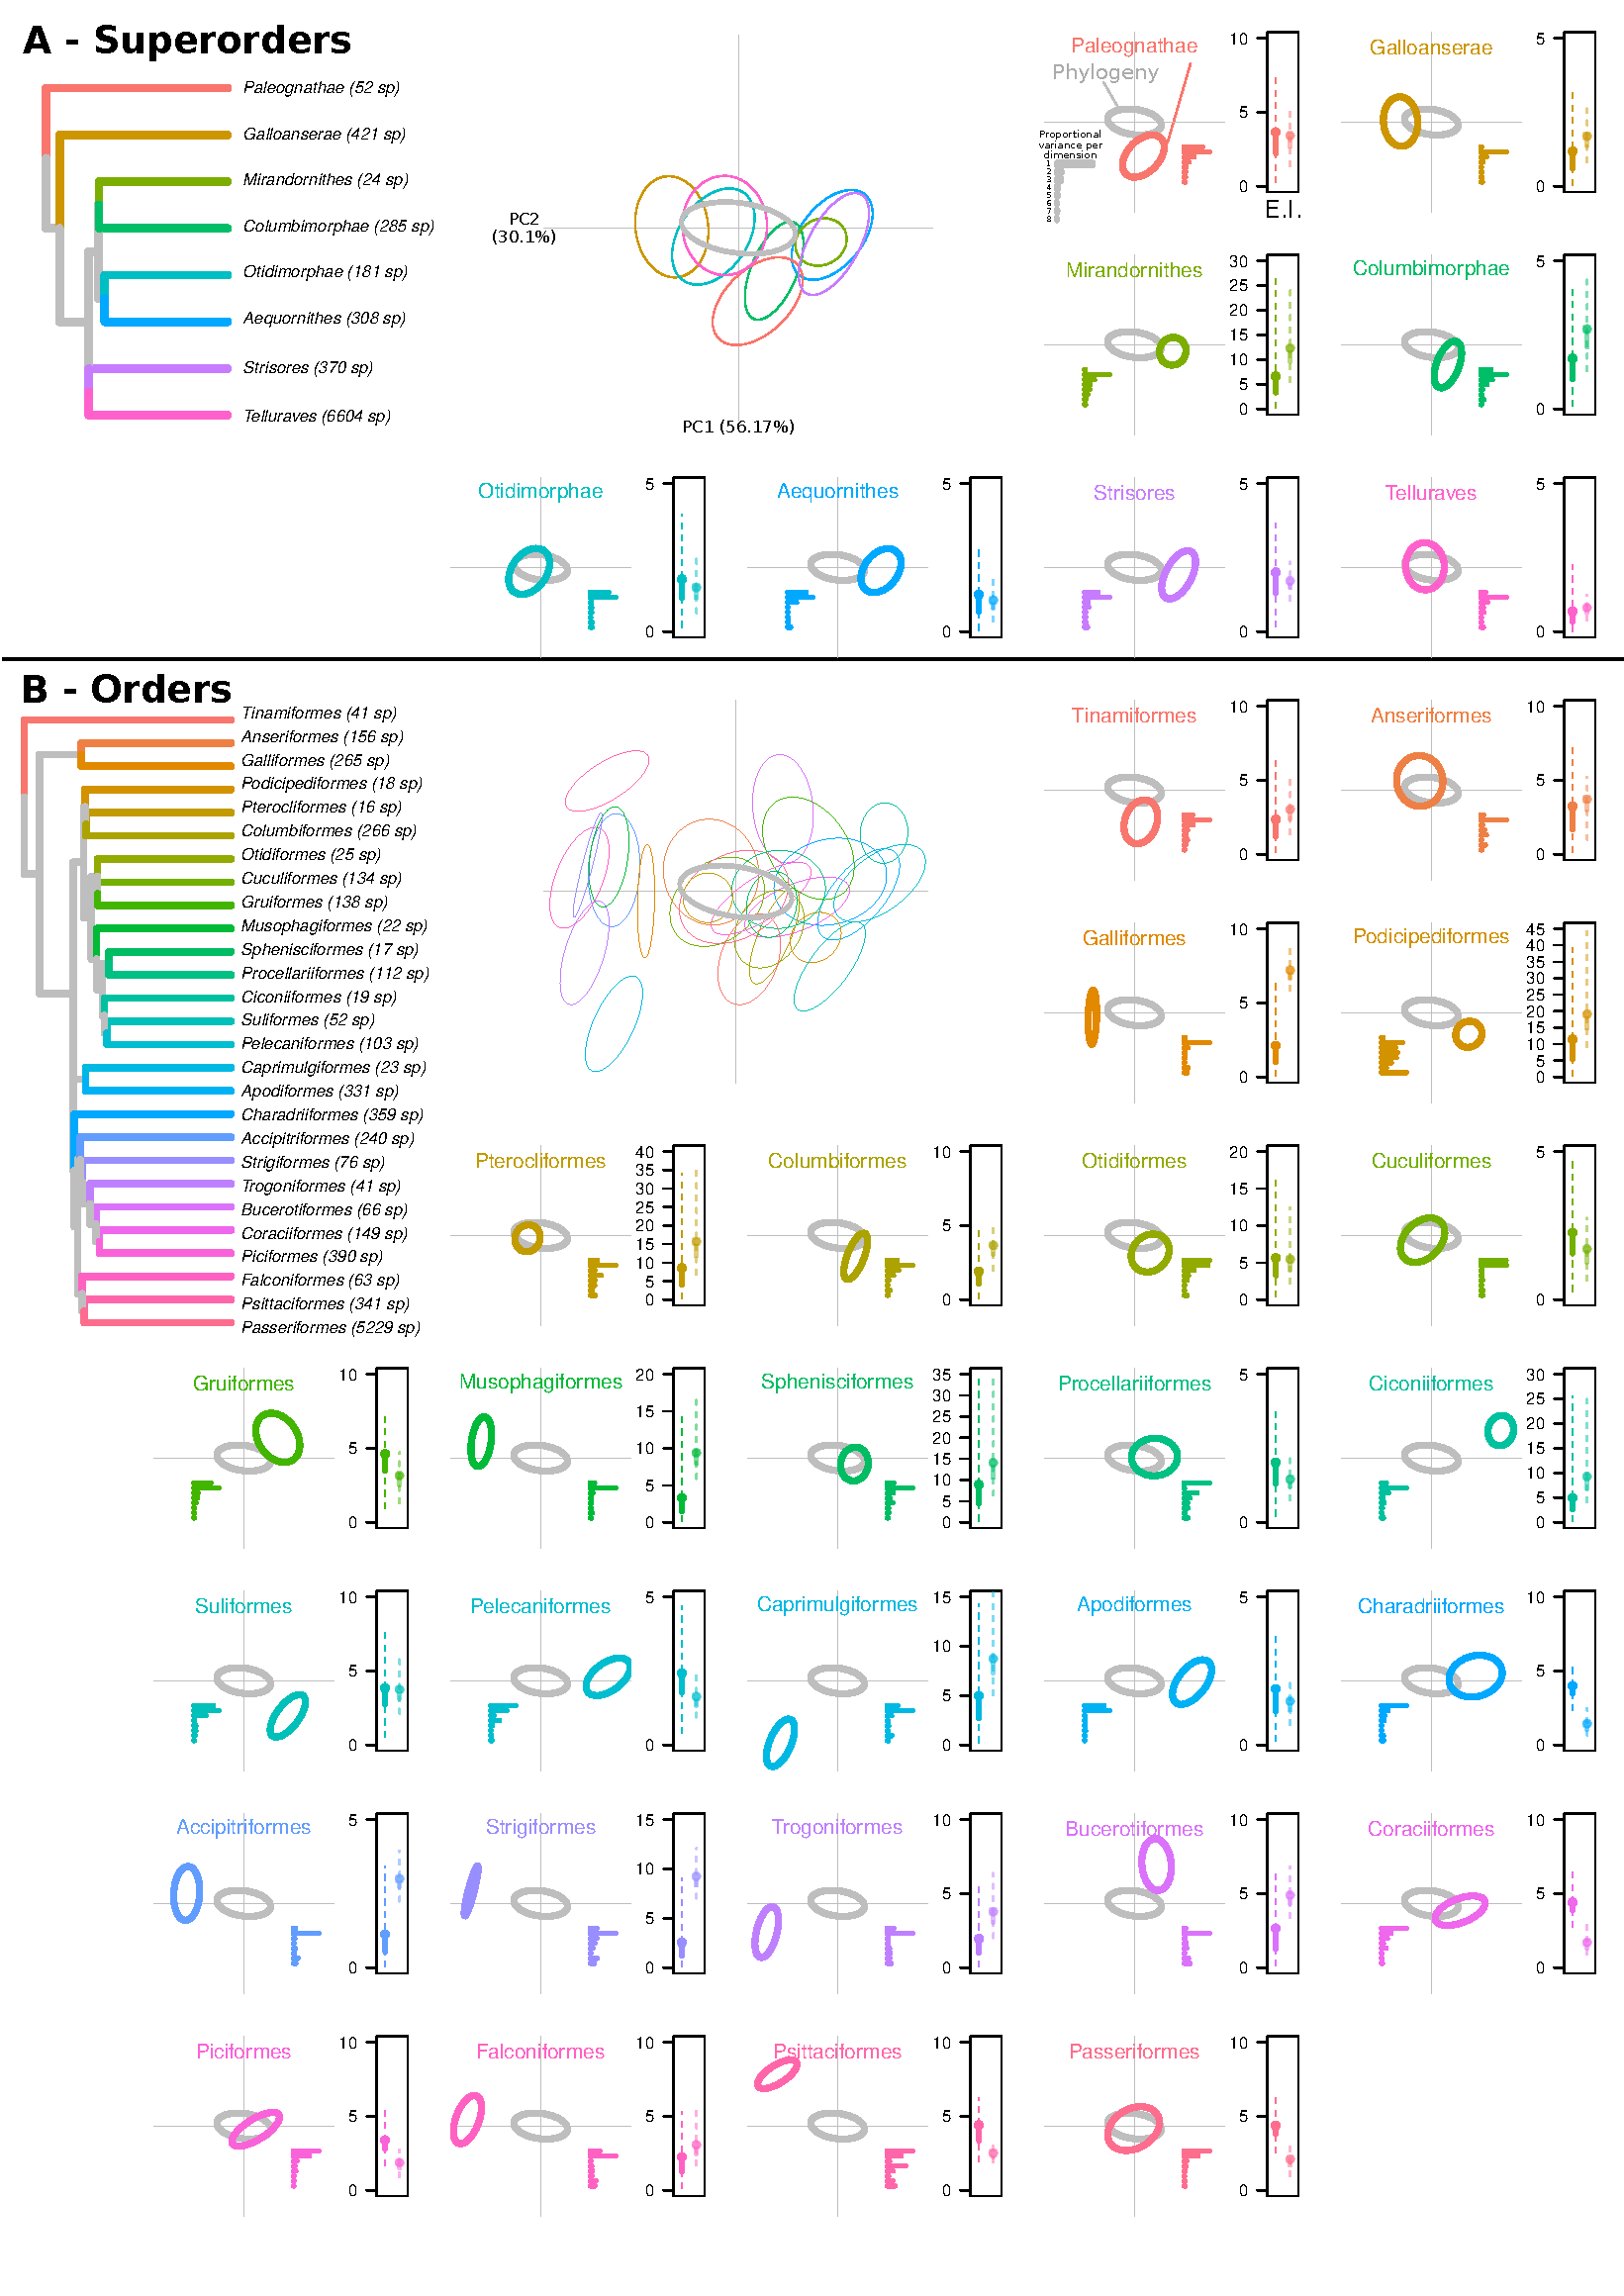
\includegraphics[width=1\textwidth]{Figures/ellipses.pdf}
\caption{.}
\label{Fig:ellipses}
\end{figure}
\bigskip

\noindent \textbf{Figure \ref{Fig:ellipses}:}
Panel A) shows  ellipses representing the scaled median posterior variance-covariance response from the pGLMM models for each superorder (coloured ellipses) compared to the all-birds phylogenetic component of the models (grey ellipses)
We scaled the ellipses so the length of the major axis of the clade ellipses is the same length as that of the global ellipse (in eight dimensions).
The first inset ellipse plot shows the positions of all superorder ellipses relative to the all-bird phylogenetic ellipse.
Subsequent inset plots show the results for each superorder. Inset barplots show the proportion of variance associated with each of the eight PC axes in shape morphospace.
The inset boxplots correspond to the elaboration (E) and innovation (I) scores for all 4000 posterior samples.
The dots represent the median elaboration and innovation values while the thick and dashed lines represent the 50\% and 95\% confidence intervals respectively.
Note that these scores were calculated on the unscaled ellipses resulting in different scales of elaboration and innovation scores for each plot. Panel B) shows  the results for each order.
A companion plot showing further nested structure within the Passeriformes is shown in Fig. S\ref{fig_ellipses_passeriformes}.

\bigskip

\begin{figure}[!htbp]
\centering
   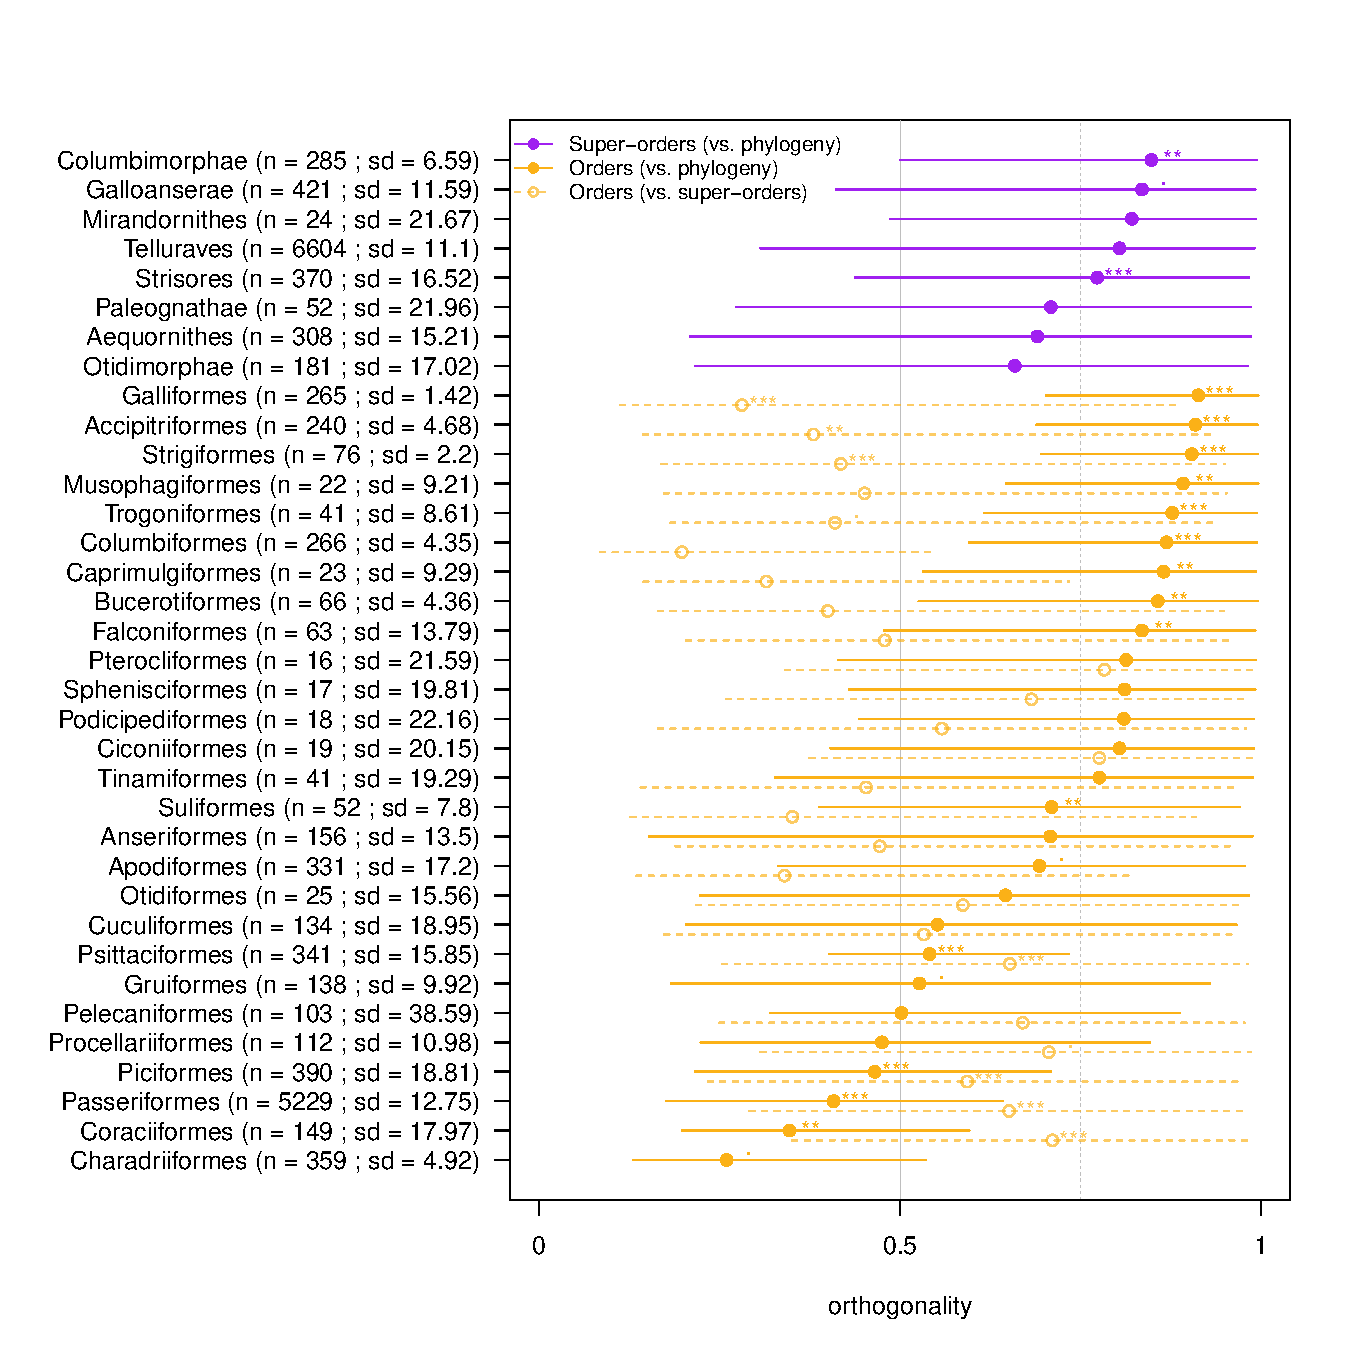
\includegraphics[width=0.9\textwidth]{Figures/orthogonality_results.pdf}
\caption{.}
\label{Fig:orthogonality}
\end{figure}

\bigskip

\noindent \textbf{Figure \ref{Fig:orthogonality}:}
Orthogonality of each clade's major axis compared to their parent or parent parent's clade.
Orthogonality is represented on the horizontal axis scales from 0 (modulo of $0^\circ$) to 1 (modulo of $90^\circ$) with the background grey and dashed grey lines represent respectively an orthogonality of 0.5 (modulo of $45^\circ$) and 0.75 (modulo of $67.5^\circ$).
Dots represent the clades median orthogonality and the lines their 95\% CI.
No super order's major axis is parallel to the whole phylogeny (red lines and circles) and 12/25 orders are at keast half orthogonal to their super-order (green lines and circles).
These results are even clearer when comparing them to the whole phylogeny (green dashed lines and open circles) where only 3/25 are not at least half orthogonal.
Furtheremore we also indicate here the number of species (n) and the standard deviation of their major axes orientation over the 4000 variance-covariance posteriors (sd; expressed in degrees).
For each clade we also measured the posterior propbabilityof each clade's orientation being different from their parent's clade or the whole phylogeny relative to their sample size and sd.
The stars represent the posterior probability of the clade's orientation being different from the comparison clade. (*** = pp $> 0.99$; ** = pp $>0.95$; * = pp $> 0.9$; . = pp $> 0.8$).
Only two out of six super-orders; 6/25 orders relative to their super order and 9/25 orders relative to the phylogeny have a pp $> 0.99$.
This is the result of a variation of sample size (n) and standard variation (sd) between clades. 
A companion plot showing further nested structure within the Passeriformes is shown in Fig. S\ref{fig_orthogonality_passeriformes}.

\bigskip

However, this change in the line of least resistance's orientation between different clade levels varies between clades (Fig.\ref{Fig:ellipses}).
While orthogonality provides a simple description of the degree of reorientation of phenotypic axes (measuring the two-dimensional plane of an angle), it does not fully capture the multi-dimensionality of the data.
To further quantify the tension implied between theory on lines of least evolutionary resistance and observations of deep-time reorientation of trait covariance, we measured the elaboration and innovation of each different clades (\textit{cf.} the elaboration and innovation of a species - see below).
As noted above, elaboration describes multivariate evolution that is primarily along the phylogenetically constrained phenotypic major axis whereas innovation describes multivariate evolution that is primarily away from the phylogenetically constrained phenotypic major axis \cite{endler2005animal}.
Clades (or species) can be both elaborators and innovators.
To measure innovation and elaboration we translated the major axes of each group's (i.e. superorders and orders) phylogenetic variance-covariance matrices onto the global phylogenetic major axis so that they shared the same origin in the shapespace.
We then used multilinear algebra to project a focal group's major axis onto the phylogenetic major axis (Fig.S\ref{Fig:cheat_sheet}).
We interpret the measured projection (distance onto the phylogenetic major axis) as the group's elaboration score and the measured rejection (distance from the major axis) as the group's innovation score.
These scores were measured for each of 4000 posterior pairs of group vs. phylogenetic variance-covariance matrix (Fig.\ref{Fig:ellipses} boxplots).
We found that for most groups the phenotypic major axis is not aligned with the global phylogenetic major axis, (Fig. \ref{Fig:ellipses}).
Remarkably, more than half of the assessed groups (4/8 superorders and 15/27 orders) displayed higher median innovation than median elaboration scores implying that, contrary to theory \cite{schluter1996adaptive,marroig2005size}, innovation is a more common generator of morphological diversity than elaboration.
However, there is substantial variation in terms of elaboration and innovation across groups including relatively low elaboration and innovation (e.g. Cuculiformes; Fig. \ref{Fig:ellipses}), low elaboration and high innovation (e.g. Galliformes; Fig. \ref{Fig:ellipses}), high elaboration and low innovation (e.g. Coraciiformes; Fig. \ref{Fig:ellipses}) or both relatively high elaboration and innovation (e.g. Podicipediformes; Fig. \ref{Fig:ellipses}).
These patterns hold across scales including within superorders and at finer scales within the order Passeriformes (Fig.S\ref{fig_ellipses_passeriformes}).
This suggests that divergence away from line of least evolutionary resistance (i.e. the phylogenetic major axis) is a common feature of avian beak evolution across scales and further supports the suggestion of a remarkable flexibility in the direction of evolution in deep-time even in a developmentally constrained trait.

This apparent lack of deep-time evolutionary constraint in bird beaks is supported by variation in both the dominant direction of evolution within clades and their relative dimensionality.
Although the major axis of the global phylogenetic component aligns closely with the first dimension (70.96\% of the phylogenetic major axis is aligned on PC1; Fig. \ref{Fig:ellipses}) of the raw shapespace, no superorder, and only seven of the 27 orders (Procellariiformes, Pelecaniformes, Charadriiformes, Coraciiformes, Psittaciformes and Passeriformes), align with PC1 in shapespace Fig. \ref{Fig:ellipses}-bar plots).
These patterns are similar (albeit more contrasted) when looking at sub-orders and families within passeriformes half off the sub-orders (Meliphagoidea, Corvides and Passerida) and seven out of the 23 families (Eurylaimides, Meliphagoidea, Petroicidea, Fringilidae, Aegithaloidea, Pyconotiae, Nectariniidae) align with PC1 (Fig. S\ref{fig_ellipses_passeriformes}).
Moreover, we found that within clades, phenotypic variation is either highly constrained (varying almost entirely along a single axis) or higher-dimensional than expected from the global phylogenetic partition.
For example, Accipitriformes (hawks and allies) have major axes that mainly align with the second dimension of the shapespace suggesting uniformity in their beak shape components, whereas the Podicipediformes (grebes) are highly variable across all dimensions suggesting that all components of the shapespace are necessary to describe their beaks.
These observations illustrate multiple routes to innovation and imply that such innovation could arise at any time throughout avian history.
However, although we see repeated innovation at the clade level, providing a new hypothesis to explain the expansion of avian morphological space, these analyses do not allow us to distinguish whether reorientation arises through abrupt changes or more gradual realignment of species in trait space.

Abrupt reorientation of trait space in higher taxa would be consistent with Simpsonian megaevolutionary dynamics \cite{simpson1953major}.
This would lead to an expectation that species should elaborate relative to their parent clade (e.g. within orders) but show a stronger tendency towards innovation relative to the global phylogeny.
To assess the relative contributions of elaboration and innovation in beak morphology among species we estimated the algebraic projection and rejection of their position in the shape-space onto (i) the global phylogenetic major phenotypic axis, (ii) the major phenotypic axis of their respective parent superorder, and (iii) the major phenotypic axis of their respective parent order.
We did this by using the same multilinear algebraic method as described above but measuring elaboration and innovation for individual species (across the 4000 posterior samples) rather than for entire groups.
We found that high levels of elaboration are more common across all birds than high levels of innovation (Fig. \ref{Fig:phylogeny}).
However, we also found various combinations of elaboration and innovation across birds.
For example, compared to the phylogenetic major axis, the Trochilidae (hummingbirds, with long narrow beaks) display high levels of elaboration and low innovation whereas the Bucerotidae (hornbills, with large and oddly shaped beaks) display high levels of innovation and low elaboration.
Other groups such as the Apodidae (swifts, with large but gaping beaks) and the distantly related but convergent Hirundidae (swallows and martins) display high levels of both elaboration and innovation.
Overall, we find no consistent evidence that innovation is either positively correlated with, or trades-off with, elaboration. %(Fig. S{#fig_correlations}). %TODO: maybe add to supp?
The variability of, and apparent disconnect between, innovation and elaboration holds whether comparisons are made at the order, superorder, or class-wide phylogenetic level (Fig. \ref{Fig:phylogeny}). %{#fig_correlations}),%TODO: maybe add to supp?
 and in further nested analysis of the order Passeriformes (Fig. S\ref{fig_ellipses_passeriformes} and S\ref{fig_phylogeny_passeriformes}).
The dominance of elaboration when measured at the species level is consistent with ideas of evolution along lines of least evolutionary resistance, yet contrasts with our observations of frequent innovation via reorientation of trait space within clades.

\begin{figure}[!htbp]
\centering
    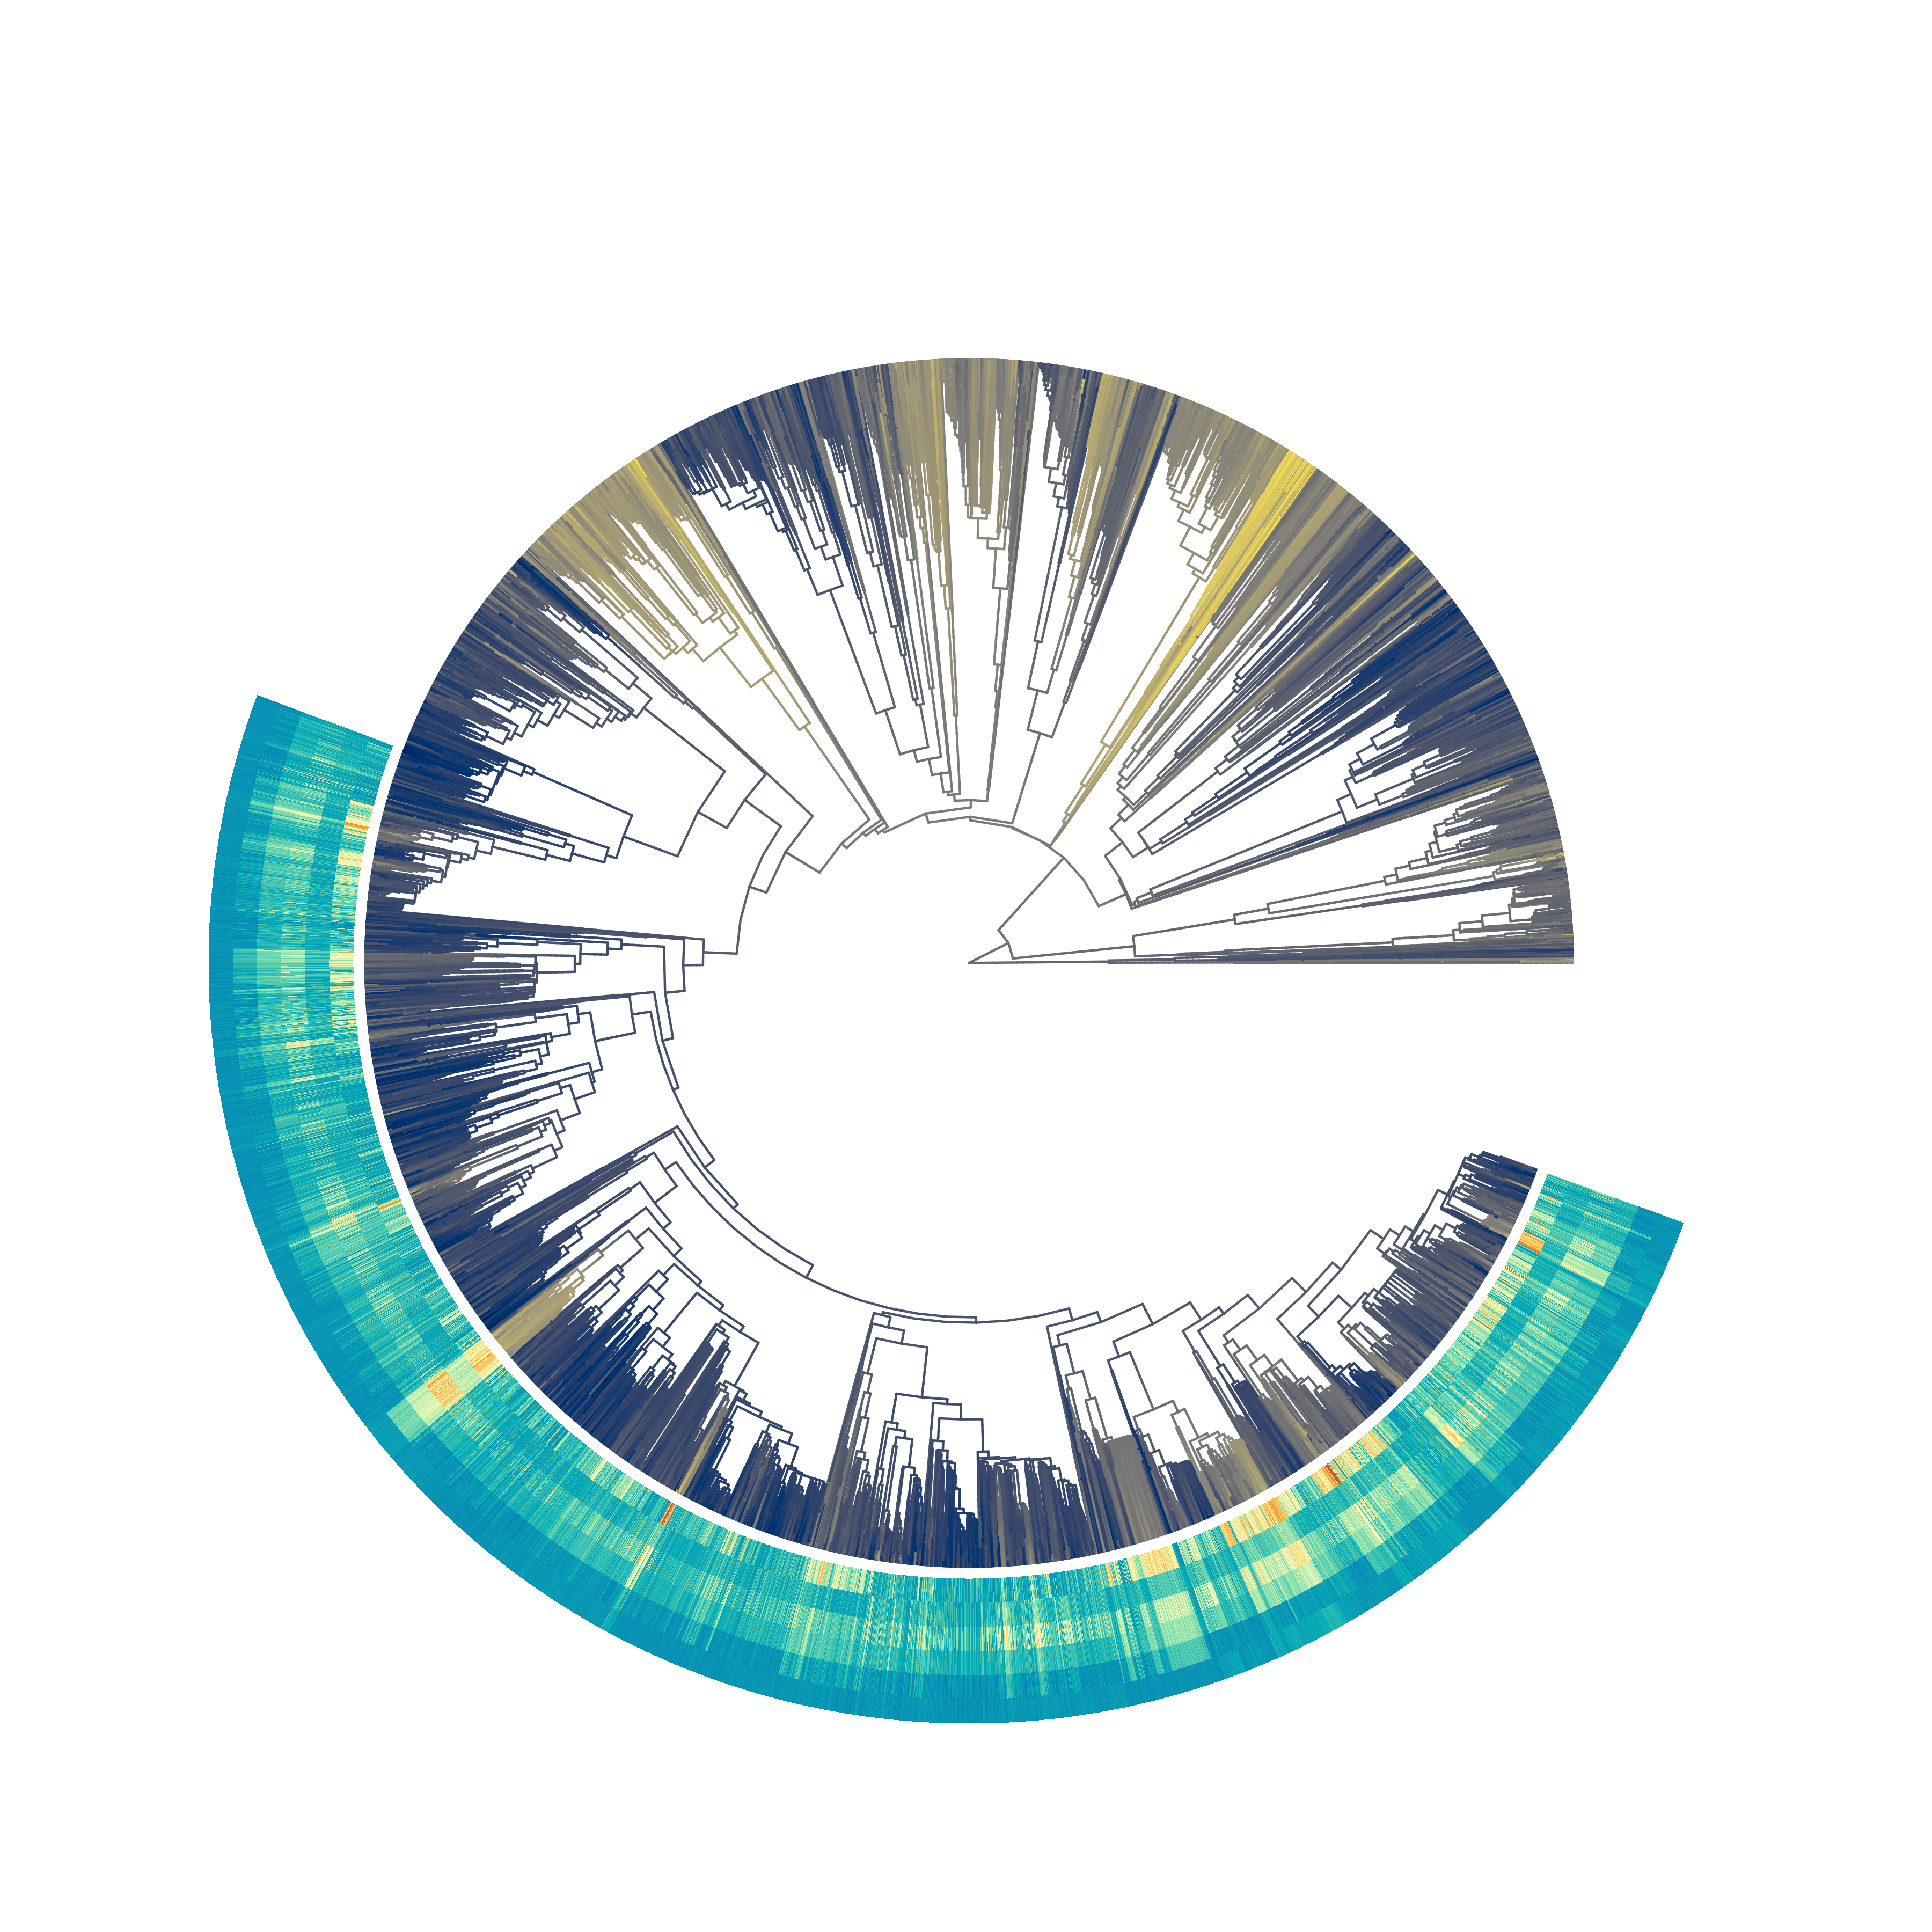
\includegraphics[width=0.9\textwidth]{Figures/InnovElabTree_main_text.pdf}
\caption{.}
\label{Fig:phylogeny}
\end{figure}

\bigskip

\noindent \textbf{Figure \ref{Fig:phylogeny}:} The avian phylogeny (n=8748 species) coloured by speciesbeak shape innovation and elaboration level.
Blue and yellow colors highlight species with relatively low elaboration or low innovation, whereas orange to red colours indicate high innovation or elaboration.
Innovations and elaboration are displayed as: a)comparisons of species to the phylogenetic major axis (inner two bands); b) comparisons of species to their superorder major axis (middle two bands); and c) comparisons of species to their order major axis (outer two bands).
The branches are coloured by the species distance from the centroid of the shapespace and the estimation of their ancestors' position in that space.
A companion plot showing further nested structure within the Passeriformes is shown in Fig. S\ref{fig_phylogeny_passeriformes}.

\bigskip

The disconnect between observations of reorientation of trait space at the clade level and a dominance of elaboration at the species level could be viewed as a paradox.
We formalise this paradox by testing whether elaboration is more common at higher taxonomic levels than at the species level.
We compared the area under the curve of the scaled density of elaboration and innovation at both the species level and the clade level.
We then measured the difference between both areas and found that there was a significant difference in innovation between species and groups but no clear difference in elaboration (Fig. \ref{Fig:relative_EI}).
This difference confirms our observation that innovation is more common at the group level rather than at the species level and that although species evolve preferentially along a line of least evolutionary resistance, this line of least resistance changes frequently among clades.
However, we suggest that rather than a paradox the reorientation of trait space can instead be described as a gradual process occuring in response to shifting selection pressures acting on species evolving in similar adaptive zones.
This implies that gradual directional evolution \cite{pagel2022general} rather than megaevolutionary jumps \cite{cooney2017mega,venditti2011multiple} may be sufficient to explain diversity in avian beak morphology.

\begin{figure}[!htbp]
\centering
   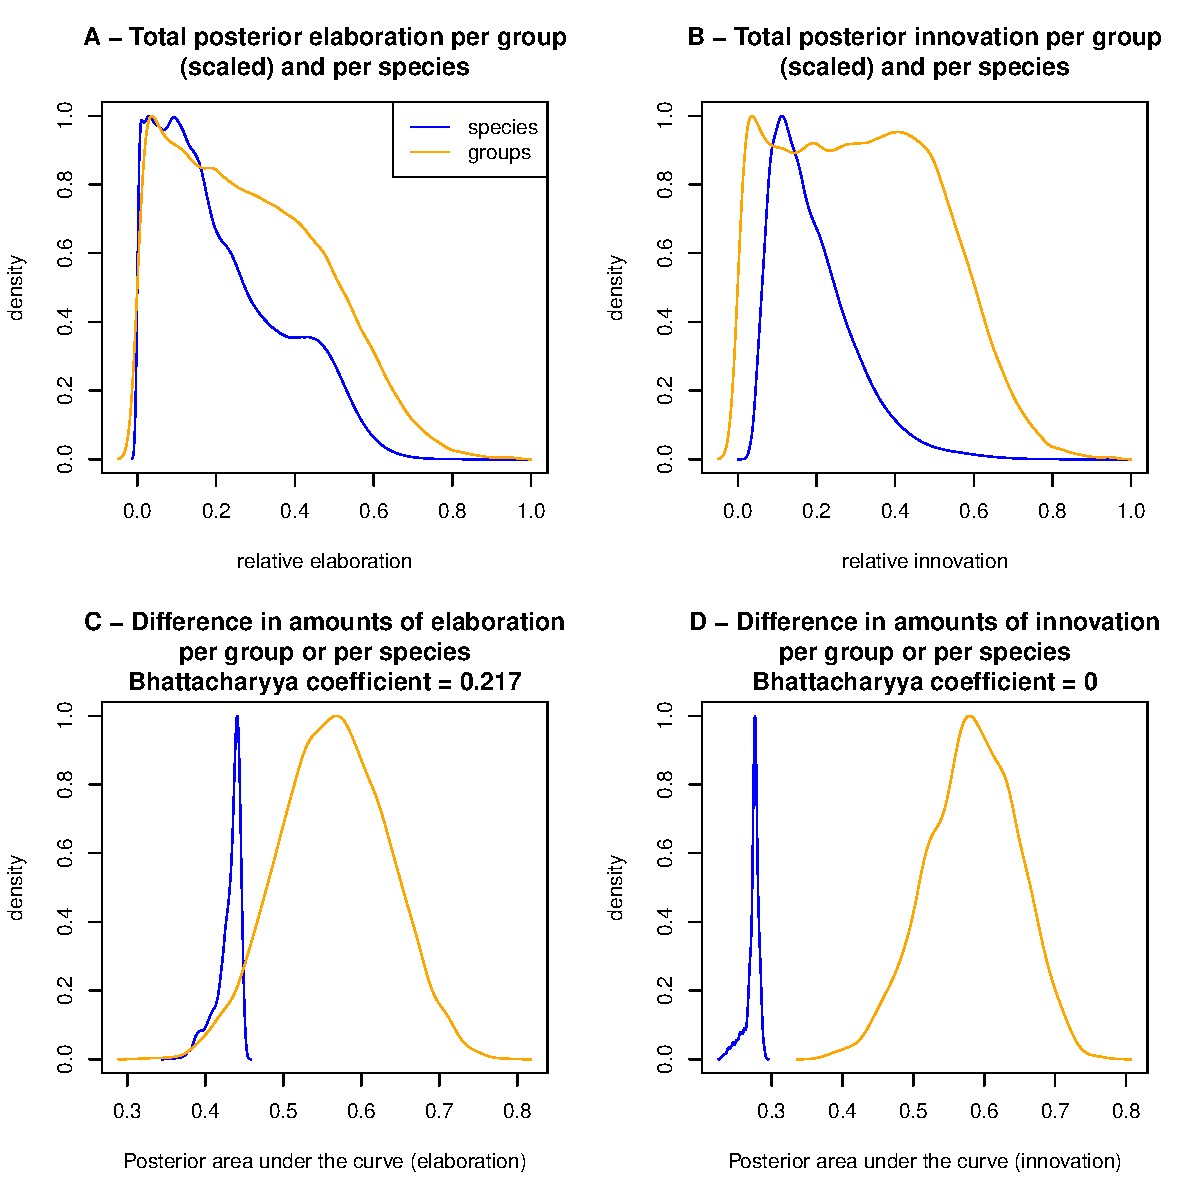
\includegraphics[width=0.9\textwidth]{Figures/relative_EI.pdf}
\caption{.}
\label{Fig:relative_EI}
\end{figure}

\bigskip

\noindent \textbf{Figure \ref{Fig:relative_EI}:} Comparisons of relative elaboration and innovation among groups (illustrated in figure  \ref{Fig:ellipses}) and among species (figure \ref{Fig:phylogeny}).
A - In blue, the elaboration for each species in each 4000 posterior samples compared to the elaboration for each 35 groups.
The scores for each group is scaled by the maximum score within each group (corresponding to the scaled ellipses in figure  \ref{Fig:ellipses}) and the score for the species is scaled by the maximum species elaboration score.
This allows us to compare both types (species vs.
groups) despite their different sample sizes.
B - same as A but for the innovation score.
C - density curve of the area under the curve for each posterior sample relative elaboration score as a proxy for the overall amount of elaboration per sample and per type (species or group - respectively blues and orange).
The Bhattacharyya coefficient indicates the probability of overlap between the posterior distributions.
D - same as C but for innovation.
We can see a clear difference in the amount of innovation across the posterior samples between species or groups.

\bigskip

Our results show that although at the species level most bird beaks are elaborating along a megaevolutionary line of least resistance, at the macroevolutionary level innovation along the megaevolutionary line of least resistance is much more common.
This nested structure of elaboration at a higher taxonomic level and innovation at a lower taxonomic level could thus explain the diversity of bird beaks we observe today.
However, individual specie-level variation in the past could also have led to a shift in a group's line of least evolutionary resistance through different evolutionary routes on a dynamic adaptive landscape, Taken together, our results suggest that the signature of evolutionary orientations in deep-time, coupled with elaboration at the species-level, is consistent with recent suggestions that the apparently abrupt phenotypic shifts can be explained by normal Darwinian processes \cite{pagel2022general}.
Our results help to bridge the gap between micro- and macro-evolution by proposing a multi-scale framework for  phenotypic evolution that allows species to evolve along lines of least evolutionary resistance while accommodating frequent shifts in the direction of evolutionary change.

\section{Methods}


\textbf{Beak shape data.}
We used the dataset from \cite{cooney2017mega,chira2020signature,hughes2022global} which consists of four landmarks and three curves of 25 semi-landmarks each, taken from 3D scans of  the beaks of 8748 bird species.
The landmark data were aligned with Procrustes superimposition using the R package \texttt{Morpho} \cite{Rcore,Morpho} and we removed the size component and controlled for symmetry (see \cite{cooney2017mega,chira2020signature,hughes2022global} for detailed descriptions of data collection and processing).
We ordinated the superimposed landmarks using a principal components analysis (PCA) and selected the first eight first dimensions of the resulting PCA.
These eight dimensions contained at least 95\% of variance in each superorder, and 98.7\% of the variance in the whole dataset.
We used a threshold of $>95$\% of variance explained for each superorder because although the overall distribution of the variance on each PC axis in the whole trait-space is decreasing (i.e.
$\sigma$ PC1 $<$ $\sigma$ PC2 $<$ $\sigma$ PC3), this is not always true for each superorder.
For example, in the Mirandornithes, PC2, then PC4, and then PC1 contained the most variance (Fig. \ref{Fig:ellipses} and S\ref{Fig:axes_variance}).
This protocol for selecting the number of PC axes ensures that the resulting trait-space contains enough variance for each superorder (see Fig. S\ref{Fig:axes_variance} and Table \ref{tab_variance_per_axis}).
This procedure resulted in an $8748 \times 8$ matrix that contains at least 95\% of the variance in all observed living bird beaks (hereafter, the shapespace).

\textbf{Phylogenetic data.}
We used a random subsample of 1000 trees from the avian tree distribution of \cite{jetz2012global} for the analyses and the one randomly selected tree for the figures (Fig. \ref{Fig:phylogeny}).
We pruned these trees to contain only the 8748 species present in our beak shapespace.




\textbf{Phylogenetic GLMM analysis.}
We ran a phylogenetic Bayesian generalised linear mixed effects model (pGLMM) using the \texttt{MCMCglmm} R package \cite{MCMCglmm} with the shapespace data as a multidimensional response variable, the error in the dataset as residuals, and each clade's phylogeny as a nested random term, i.e., a model of:

\begin{equation}
\text{shapespace} \mathtt{\sim} \text{residuals(shapespace)} + \text{random(phylogeny)} (equation 1)
\end{equation}

This model allows us to estimate a phenetic variance-covariance matrix for each clade and the phylogeny as a whole, and one for the residuals in the shapespace itself \cite{robinson2013quantifying}.
These variance-covariance matrices were then used in a base projection-rejection analysis to measure the elaboration and innovation scores (see below).
We ran two separate nested models.
One model using one random term for the whole phylogeny and 35 nested random terms for each superorder and order containing more than 15 species in our dataset (Fig. \ref{Fig:ellipses}).
And one model on a subset of the dataset containing only the 5966 passeriformes species with 30 nested random terms.
This resulted in two multidimensional GLMM.
One with a $8748 \times 8$ response variables, one global residual term and 36 random terms.
And one with a $5966 \times 8$ response variable, one global residual term and 30 random terms.
 
To account for phylogenetic uncertainty we needed to run the model using different tree topologies from the tree distribution in \cite{jetz2012global}.
Because of the very large size of our model and dataset, however, running the full model on multiple trees was computationally unfeasible (it would require 2 CPU years and 4TB of RAM for each - the whole tree and the passeriformes ones).
Instead, we developed and implemented a ''mini chains'' MCMCglmm method using the R package \texttt{mcmcmglmmm} \cite{mcmcmcglmmm}.

\textbf{mcmcmcglmm.}
This method consists in running relatively short monte-carlo markov chains (MCMC) across a large number of different phylogenetic trees and concatenating the resulting short posteriors into one larger one that contains the phylogenetic uncertainty information.
This was effectively done in four steps (see Fig. S\ref{Fig:mcmcmcglmm})
1) running three independent MCMCglmm chains (hereafter the parametrisation chains) for 50k generations with the traits data and the model described above on the consensus tree from the tree distribution, along with flat priors with a belief parameter of 2\% (effectively not a very low weight on the priors);
2) extracting the following parameters from the parameterisation chains:
a) the conservative burnin average time (across the three chains) defined as the highest number of iterations required to first reach the median posterior likelihood value multiplied by 1.1; and
b) the mini-chains priors defined as the median posterior model values from the parameterisation chains with a belief parameter of 5\%.
We then ran 400 mini chains in parallel with the estimated burnin time and priors in order to just run 10 samples past the burnin.
This effectively resulted in getting 10 exploitable posterior samples per tree.
We used 400 trees because that was the number of models required to reach an effective sample size (ESS) of at least 200 for all the estimated parameters (see Fig. S\ref{Fig:model_ess_all_birds} and S\ref{Fig:model_ess_passeriformes}).
Using this approach, we reduced the computational time to around 45 CPU hours and 9GB of RAM per mini-chain (a 400 fold improvement).
The whole procedure is reproducible in the \href{https://raw.rawgit.net/TGuillerme/mcmcmcglmmm/main/inst/MCMCglmm_mini_chains.html}{\texttt{mcmcmcglmmm} vignette} \cite{mcmcmcglmmm}.

\textbf{Projection/rejection analyses.}
We used the distributions of the 4000 posterior variance-covariance matrices to run the projection/rejection analyses to measure the bird beaks' elaboration and innovation scores.
In fact we can use multilinear algebra to interpret elaboration and innovation \textit{sensu} \cite{endler2005animal} by using the major axis of the variance-covariance matrices as the ''line of least resistance'', or, specifically here, the line of elaboration for each random terms (corresponding to the elaboration axes for each clade) and project either species or other major axis onto that group.
In brief we can interpret where a species or a group falls on the major axis of reference as its elaboration score and how far a species is from that major axis as its innovation score.
We calculated the elaboration and innovation scores using two main approaches:
1) by clades (i.e. to measure the elaboration/innovation between clades) where we calculated the projections of the major axes of each clade onto the global phylogenetic major axes (Fig. \ref{Fig:ellipses});
and 2) by species (i.e. to measure the elaboration/innovation within clades) where we calculated the projections of each species onto a) the global phylogenetic major axes and b) the phylogenetic major axes of their respective clade (Fig. \ref{Fig:phylogeny}).
To make the results easier to interpret, we centered and scaled them onto the centre of the major axis of interest and made the elaboration values absolute.
This way, we can interpret an elaboration or innovation score within the 0-1 range to be not exceptional (i.e within the 95\% confidence interval of the variance-covariance matrix).
The entire mathematical procedure is described in details in the supplementary materials (section \ref{supp_projection}).
The whole procedure applied to our dataset is reproducible in \href{https://raw.rawgit.net/TGuillerme/dispRity/master/inst/vignettes/Projection_analysis.html}{this \texttt{dispRity} vignette} % TODO: update link to release when releasing
and implemented in the dispRity package \cite{dispRity}.

\textbf{Groups' orthogonality.}
We measured the orthogonality of each group (i.e. random term in our models compared to their parent group and their parent parent's (e.g.
the Columbimorphae random terms' variance-covariance matrices against the phylogeny ones, the Columbiformes ones against the Columbimorphae ones (parent) and the whole phylogeny ones (parent parents).To do so we measured the angles between the major axes of the focal group and their parent group for each posterior variance-covariance matrix as well as within each group by randomly comparing major axes within a group.
We converted each angle measurement into an orthogonality metric where 0 corresponds to flat angles ($0^\circ$ or  $180^\circ$) and 1 to right angles ($90^\circ$ or $270^\circ$).
We then measured the posterior probability of the angles within a group being different than the angles between groups.
These results are available in Fig. \ref{Fig:orthogonality}.

\textbf{Reproducibility and repeatability.}
The raw and processed data used in this analysis is available from \href{https://figshare.com/articles/dataset/Innovation_and_elaboration_on_the_avian_tree_of_life/20480355}{figshare} \cite{fighsaredata}.
The code used to reproduce the figures and tables is available from \href{https://github.com/TGuillerme/elaboration_exploration_bird_beaks}{github} \cite{githubrepo}.

\textbf{Funding.}
This work was funded by UKRI-NERC Grant NE/T000139/1 and a Royal Society University Research Fellowship (URF R 180006 to GHT).


\bibliographystyle{naturemag}
\bibliography{references}


\end{document}